\documentclass[handout]{mcs}

\begin{document}

\microquiz{Feb. 22}

%%%%%%%%%%%%%%%%%%%%%%%%%%%%%%%%%%%%%%%%%%%%%%%%%%%%%%%%%%%%%%%%%%%%%
% Problems start here
%%%%%%%%%%%%%%%%%%%%%%%%%%%%%%%%%%%%%%%%%%%%%%%%%%%%%%%%%%%%%%%%%%%%%

\begin{problem}
Figure \ref{fig:img} shows the arrow diagram for a relation, $R$.

\begin{figure}[h]

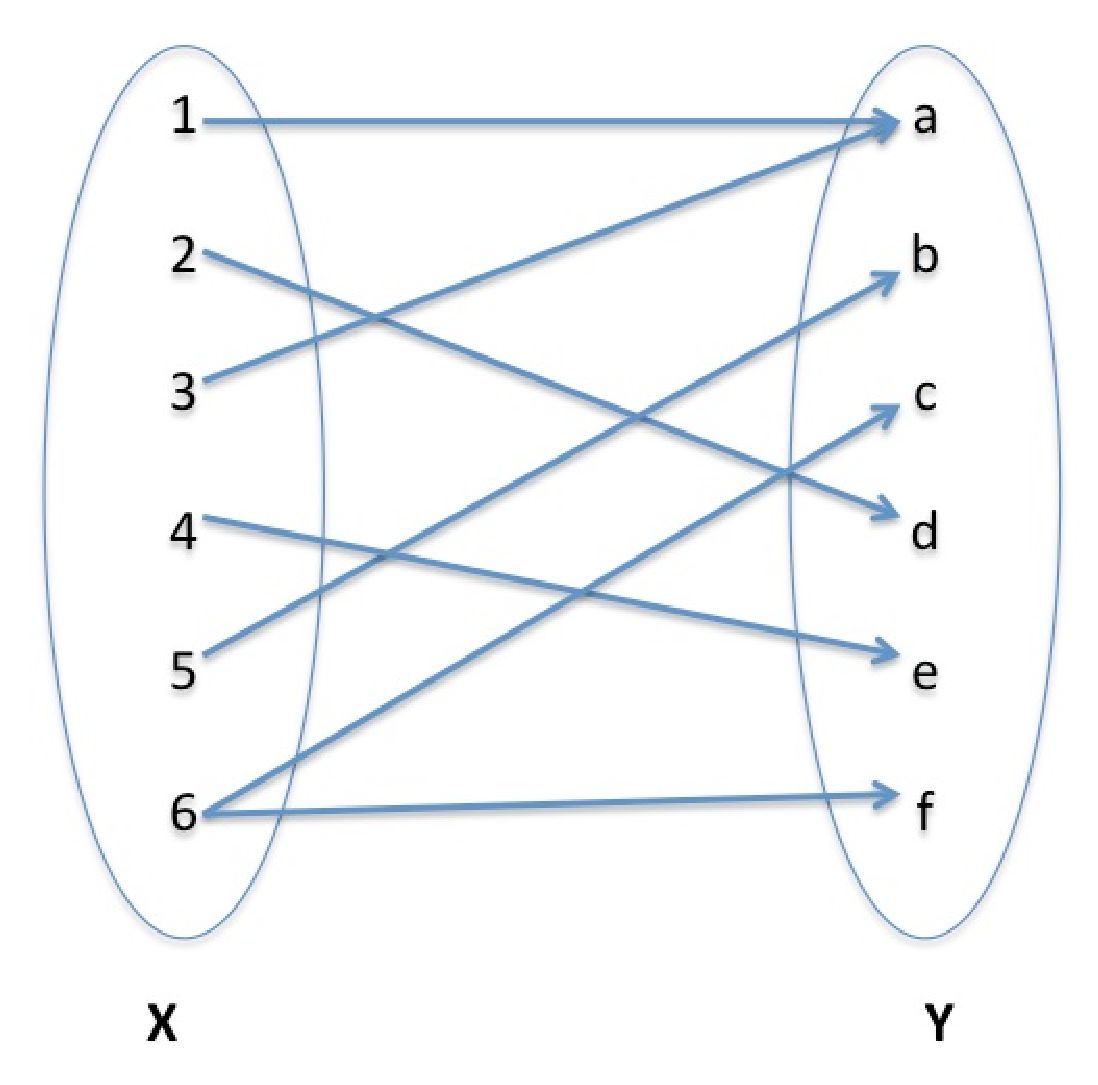
\includegraphics[height = 2in ]{image-inverseimage1}

\caption{Relation $R$.}
\label{fig:img}
\end{figure}
\bparts

\ppart List the elements in the image under $R$ of the even numbers in domain $X$.\hfill\brule{1.5in}

\ppart List the elements in the inverse image under $R$ of the vowels in codomain $Y$.\hfill\brule{1.5in}

\ppart List the first letters of \emph{all} the properties below
satisfied by relation $R$.\hfill\brule{1.0in}
\begin{center}
 \textbf{f}unction ($[\le 1\ \text{out}]$)\qquad \textbf{t}otal ($[\ge
   1\ \text{out}]$)

 \textbf{i}njective ($[\le 1\ \text{in}]$)\qquad \textbf{s}urjective
 ($[\ge 1\ \text{in}]$)\qquad \textbf{b}ijective ($[= 1\ \text{in, } =
   1\ \text{out}]$)
\end{center}

\eparts
\end{problem}

\begin{problem}
Let $A$ be the set of Albert's arms and legs, $E$ the set of Albert's
eyes, $T$ the set of Albert's toes, and $F$ the set of Albert's
fingers.  For each of the following pairs of sets, write \textbf{B} to
indicate the bij relation holds between them, \textbf{S} to indicate
the surj relation but not the bij relation, and \textbf{I} to indicate
the inj relation but not the bij relation.
\bparts
\ppart $T$\brule{0.3in}$A$.
%\ppart $A$\brule{0.3in}$T$.
\ppart $T$\brule{0.3in}$E$.
\ppart $T$\brule{0.3in}$F$.
\eparts
\end{problem}
%%%%%%%%%%%%%%%%%%%%%%%%%%%%%%%%%%%%%%%%%%%%%%%%%%%%%%%%%%%%%%%%%%%%%
% Problems end here
%%%%%%%%%%%%%%%%%%%%%%%%%%%%%%%%%%%%%%%%%%%%%%%%%%%%%%%%%%%%%%%%%%%%%
\end{document}
